% !TEX program = pdflatex
\documentclass{article}
\usepackage{tikz}
\usetikzlibrary{angles,quotes}

\begin{document}
\section*{Survey of a corner brace}
\begin{figure}[ht]\centering
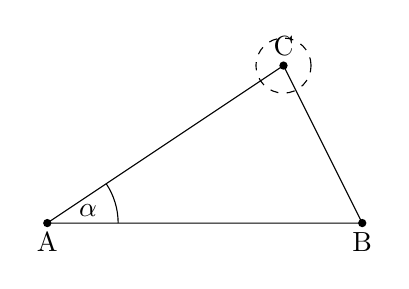
\begin{tikzpicture}

\coordinate (A) at (0,0);\coordinate (B) at (4,0);\coordinate (C) at (3,2);
\draw (A)--(B)--(C)--cycle;
\draw[dashed] (C) circle (.35);
\pic[draw,angle radius=9mm,"$\alpha$"{angle eccentricity=1.4}] {angle=B--A--C};
\foreach \p/\side in {A/below,B/below,C/above} \fill (\p) circle (1.5pt) node[\side] {\p};
\end{tikzpicture}\caption{The dashed circle marks clearance around the upper pin.}\end{figure}
\end{document}
